% ============================================================
%  Section 6: Fine-Tuning
% ============================================================

\section{Fine-Tuning}
\label{sec:finetuning}

Fine-tuning adapts the pre-trained \bert{} model to a specific downstream task by
appending a lightweight task-specific head and training \emph{all} parameters
end-to-end on labelled task data.  This stands in contrast to \emph{feature-based}
approaches (e.g., ELMo) that freeze the pre-trained encoder and use its
representations as static features.

\subsection{General Procedure}
\label{subsec:ft_procedure}

Fine-tuning proceeds as follows:
\begin{enumerate}
  \item Initialise the model with the pre-trained \bert{} weights.
  \item Construct the task-appropriate input format, inserting \cls{} and \sep{}
        tokens as required.
  \item Append a task-specific output head (typically one or two linear layers)
        on top of the relevant \bert{} output representation.
  \item Train the full model (encoder + head) jointly on the labelled training set
        using a small learning rate (typically $2\text{--}5 \times 10^{-5}$) for a
        small number of epochs (typically 3--5).
\end{enumerate}

The key advantages of this approach are its simplicity and its modest data
requirements: even with a few thousand labelled examples, fine-tuned \bert{} often
surpasses task-specific architectures trained on orders of magnitude more data.

\subsection{Task Formulations}
\label{subsec:ft_tasks}

\subsubsection{Single-Sentence Classification}
\label{ssubsec:cls}

Tasks such as sentiment analysis (SST-2) and linguistic acceptability
(CoLA)~\cite{wang2018glue} use a single sentence as input.  The final hidden state
of \cls{} is passed to a linear classifier:
\begin{equation}
  \hat{y} = \softmax(\mathbf{W}_c\,\mathbf{h}_{\cls}^{(L)} + \mathbf{b}_c),
  \label{eq:cls}
\end{equation}
where $\mathbf{W}_c \in \R^{|\mathcal{Y}| \times d}$ and $\mathcal{Y}$ is the
label set.

\subsubsection{Sentence-Pair Classification}
\label{ssubsec:pair_cls}

Tasks such as Natural Language Inference (MNLI), paraphrase detection (MRPC), and
semantic similarity (STS-B) receive a sentence pair~$(A, B)$ formatted as:
\[
  \texttt{[CLS]}\ A\ \texttt{[SEP]}\ B\ \texttt{[SEP]}.
\]
The \cls{} representation aggregates cross-sentence information through
bidirectional attention and is classified as above.

\subsubsection{Question Answering (Extractive)}
\label{ssubsec:qa}

For extractive QA tasks such as SQuAD~v1.1~\cite{rajpurkar2016squad}, the
question and passage are concatenated as the sentence pair, and the model predicts
a contiguous \emph{answer span} $(s, e)$ within the passage.  Two learned vectors
$\mathbf{w}_s, \mathbf{w}_e \in \R^d$ compute start and end logits over all
passage tokens:
\begin{equation}
  P_s(i) = \frac{\exp(\mathbf{w}_s^\top \mathbf{h}_i^{(L)})}
                 {\sum_j \exp(\mathbf{w}_s^\top \mathbf{h}_j^{(L)})}, \quad
  P_e(i) = \frac{\exp(\mathbf{w}_e^\top \mathbf{h}_i^{(L)})}
                 {\sum_j \exp(\mathbf{w}_e^\top \mathbf{h}_j^{(L)})}.
  \label{eq:qa}
\end{equation}
The predicted span is $\arg\max_{s \leq e}\, P_s(s) \cdot P_e(e)$.

\subsubsection{Named Entity Recognition (NER)}
\label{ssubsec:ner}

For sequence labelling tasks (e.g., CoNLL-2003 NER), a linear classification
layer is applied to \emph{every} token's final hidden state independently, yielding
per-token label probabilities.  The \cls{} and \sep{} tokens are excluded from the
loss computation.

\begin{table}[H]
  \centering
  \caption{\bert{} fine-tuning results on representative NLU benchmarks.  GLUE is
           a composite score; others report default metrics (Acc = accuracy,
           F1 = harmonic mean).}
  \label{tab:finetuning_results}
  \renewcommand{\arraystretch}{1.35}
  \begin{tabular}{lcccc}
    \toprule
    \textbf{Task} & \textbf{Type} & \textbf{Train Size} & \textbf{Metric} & \textbf{BERT-Base} \\
    \midrule
    MNLI & Sentence-pair (3-way) & 393K & Acc & 84.6\% \\
    QQP & Paraphrase detection & 364K & Acc/F1 & 91.3\%/88.2\% \\
    MRPC & Paraphrase & 3.7K & Acc/F1 & 89.3\%/85.4\% \\
    SST-2 & Sentiment (2-way) & 67K & Acc & 93.2\% \\
    SQuAD v1.1 & Extractive QA & 88K & F1/EM & 88.5\%/80.8\% \\
    CoNLL-2003 & NER (token-level) & 15K sent & F1 & 96.4\% \\
    \bottomrule
  \end{tabular}
\end{table}

\begin{figure}[H]
  \centering
  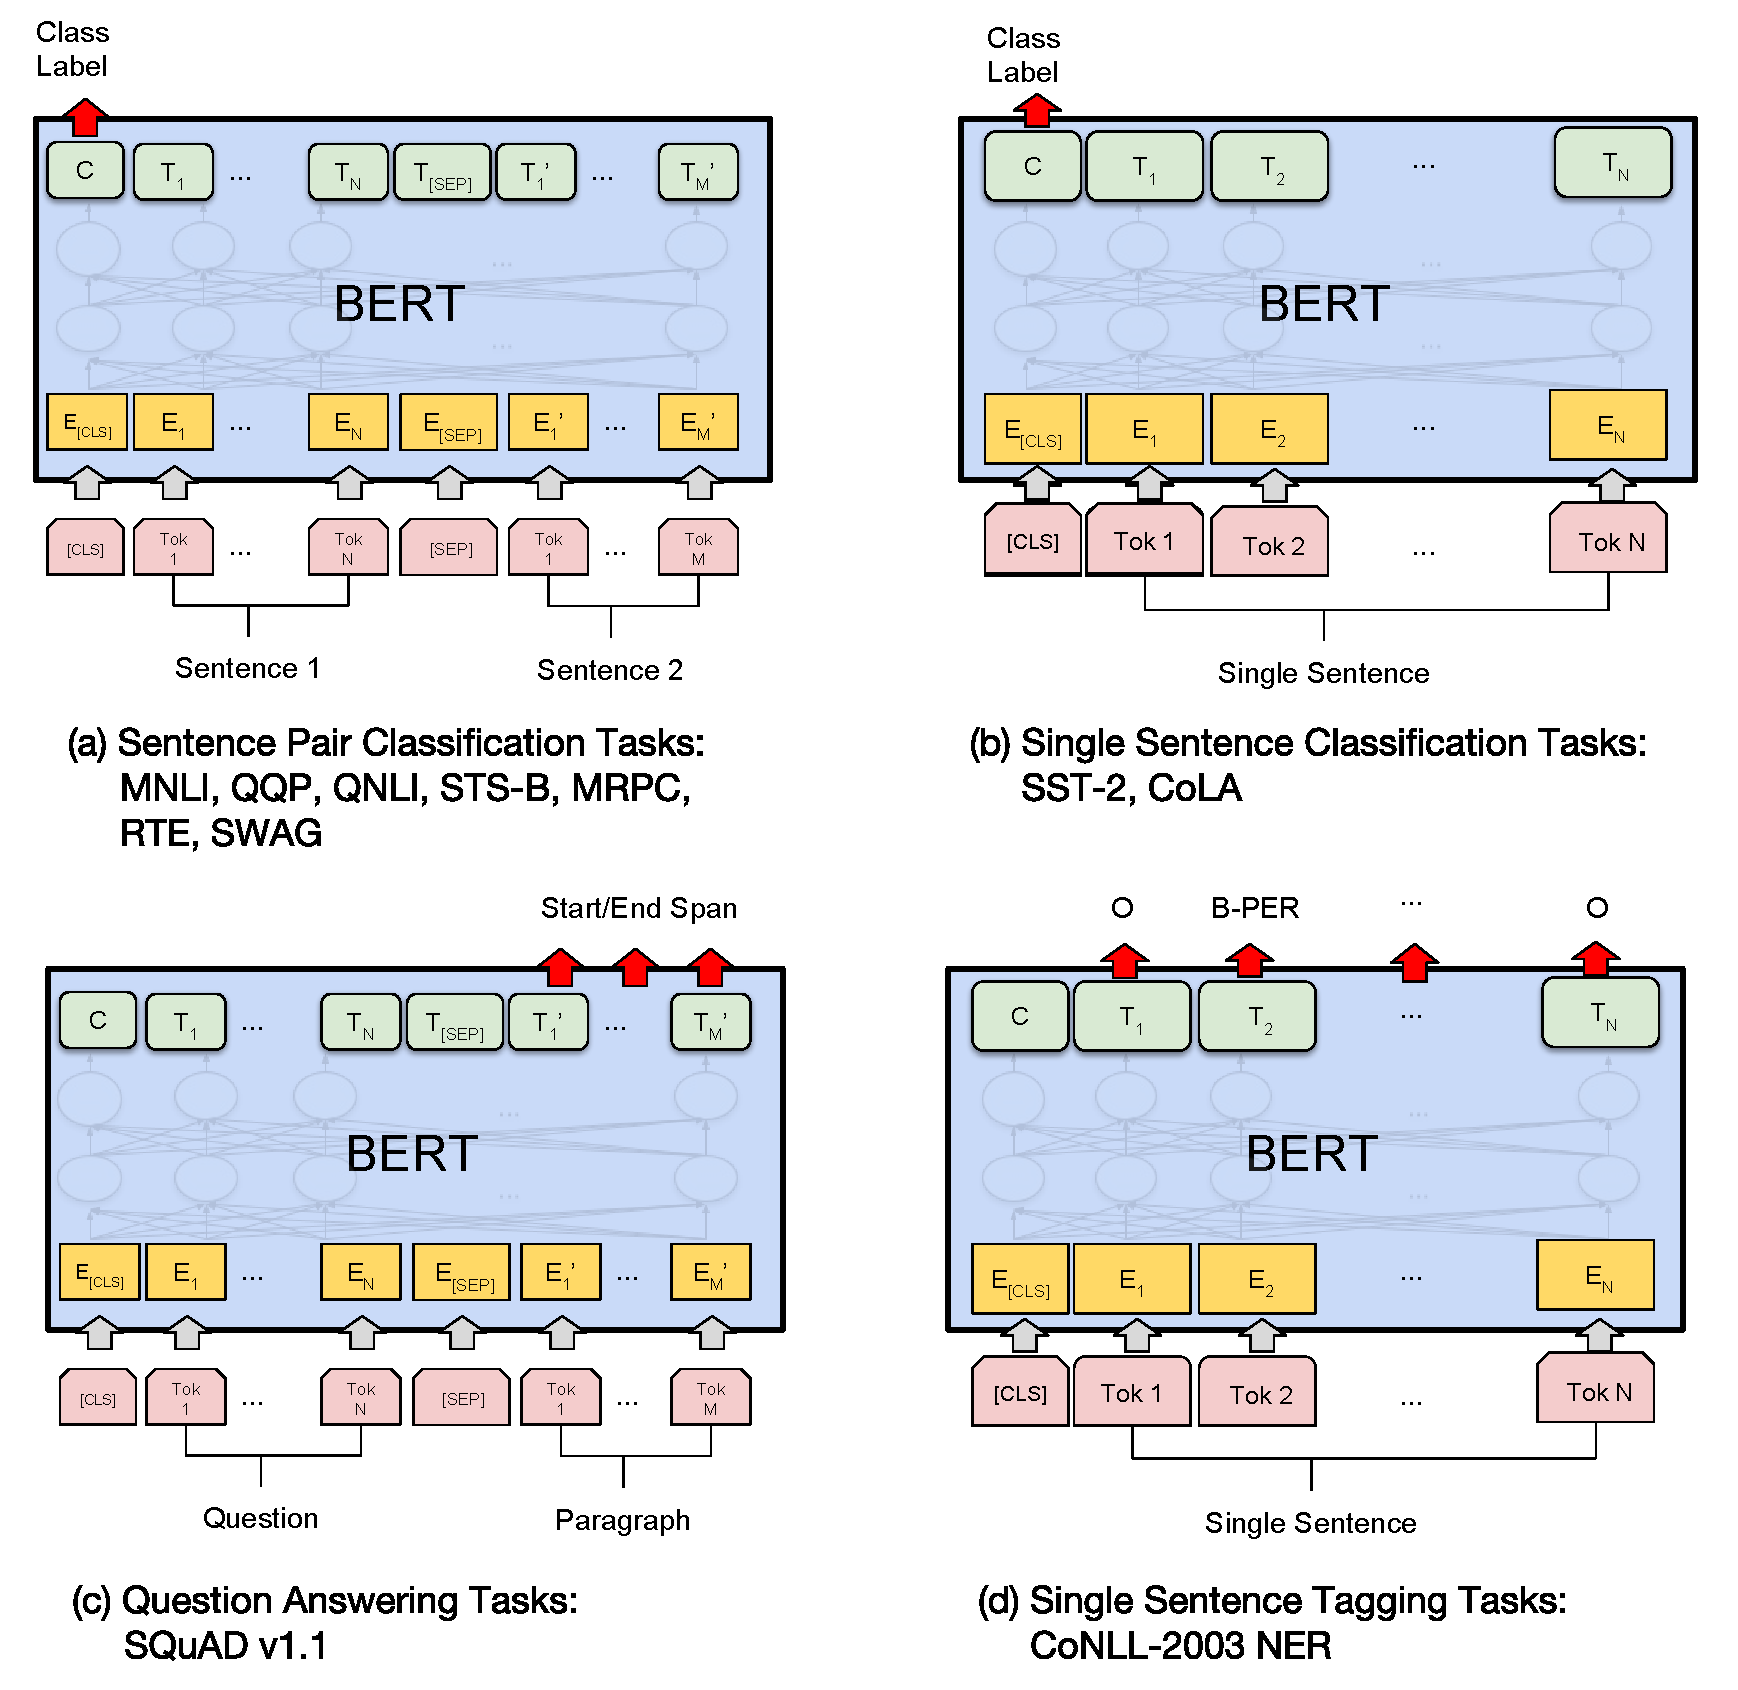
\includegraphics[width=0.90\textwidth]{figures/finetuning.pdf}
  \caption{\bert{} fine-tuning architectures for four task types.  (a)~Sentence-pair
           classification; (b)~single-sentence classification;
           (c)~extractive question answering; (d)~sequence labelling (NER).
           Only the top-layer head changes across tasks; the encoder is shared.}
  \label{fig:finetuning}
\end{figure}

\subsection{Practical Considerations}
\label{subsec:ft_practical}

\begin{itemize}
  \item \textbf{Learning rate warm-up.}  A linear warm-up over the first
        $10\%$ of training steps followed by linear decay is recommended to
        prevent catastrophic forgetting of pre-trained knowledge.
  \item \textbf{Batch size.}  Larger batch sizes (32--128) generally improve
        stability on small datasets; gradient accumulation can approximate large
        batches on memory-constrained hardware.
  \item \textbf{Layer-wise learning rate decay.}  Assigning lower learning rates
        to lower encoder layers and higher rates to the task head has been
        reported to improve fine-tuning stability~\cite{sun2019fine}.
\end{itemize}
